\documentclass{article}
\usepackage[italian]{babel}
\usepackage[tmargin=2cm,rmargin=1.5in,lmargin=1.5in,margin=0.85in,bmargin=2cm,footskip=.2in]{geometry}
\usepackage{siunitx}
\sisetup{separate-uncertainty=true, per-mode=fraction, parse-numbers=true}
\usepackage{caption}
\usepackage[T1]{fontenc}
\usepackage{bookmark}
\usepackage{graphicx}
\usepackage{multicol}
\usepackage{booktabs}
\usepackage{amsmath,amsfonts,amsthm,amssymb,mathtools}
\hypersetup{
	pdftitle={Appunti Tomadin},
	colorlinks=true, linkcolor=doc!90,
	bookmarksnumbered=true,
	bookmarksopen=true
}
\usepackage{blindtext}
\usepackage{wrapfig}
\usepackage{listings}
\usepackage{xcolor}
\usepackage{float}
\usepackage{tikz}
\usepackage{multirow}
\usepackage{biblatex}
\definecolor{codegreen}{rgb}{0,0.6,0}
\definecolor{codegray}{rgb}{0.5,0.5,0.5}
\definecolor{codepurple}{rgb}{0.58,0,0.82}
\definecolor{backcolour}{rgb}{0.95,0.95,0.92}
\definecolor{doc}{rgb}{0,0,0}
\lstdefinestyle{code}{
    backgroundcolor=\color{backcolour},   
    commentstyle=\color{codegreen},
    keywordstyle=\color{magenta},
    numberstyle=\tiny\color{codegray},
    stringstyle=\color{codepurple},
    basicstyle=\ttfamily\footnotesize,
    breakatwhitespace=false,         
    breaklines=true,                 
    captionpos=b,                    
    keepspaces=true,                                     
    showspaces=false,                
    showstringspaces=false,
    showtabs=false,                  
    tabsize=2,
    inputencoding=ansinew,
    extendedchars=true,
    numbers=left,                    
    numbersep=5pt
}

\lstset{style=code}
\usepackage[varbb]{newpxmath}
\usepackage{circuitikz}
\author{Aiello Giosuè, Fenili Domenico, Sermi Francesco}
\date{\today}
\title{Relazione conducibilità termica}

\begin{document}
\maketitle
\newpage

\tableofcontents

\newpage

\section{Scopo}

Ricavare la conducibilità termica di differenti materiali dalle misurazioni di temperatura compiute

\section{Premesse teoriche}

Dalla teoria sappiamo che la quantità di calore che si trasmette per conduzione nell'unità di tempo è pari a
\begin{equation}
	W = \frac{dQ}{dt}
\end{equation}
è detta \emph{flusso di calore} e nel sistema MKS si misura in \unit{W}. All'equilibrio termico si osserva che il flusso di calore che attraversa la barra risulta costante e, se denotiamo con $S$ la sezione della barra, $T$ la temperatura ed $x$ la posizione lungo la barra; abbiamo che:
\begin{equation}
	W = -\lambda S \frac{\Delta T}{\Delta x}
\end{equation}
dove la costante di proporzionalità $\lambda$ viene detta \emph{conducibilità termica} del materiale. Se fissiamo l'origine delle ascisse in $x_0$, abbiamo che
\begin{equation}
	W = -\lambda S \frac{T_i - T_0}{x_i}
\end{equation}
ovvero
\begin{equation}
	T_i = T_0 - \frac{W}{\lambda S}x_i
\end{equation}
Sappiamo inoltre che, per effetto Joule, la potenza dissipata come calore è pari a
\begin{equation}
	W = VI
\end{equation}
Per calcolare la conducibilità sfrutteremo il fatto che, ipotizzando l'assenza di perdite, vale la relazione
\begin{equation}
	T_i = T_0 - \frac{VI}{2 \lambda S}x_i
	\label{eq:modello}
\end{equation}
dove poniamo che $W$ sia pari a $\frac{VI}{2}$ siccome stiamo operando con un circuito con due termistori uguali in parallelo.

\section{Strumenti e materiali utilizzati}

\textbf{Materiali:}
\begin{itemize}
	\item Due barre cilindriche;
	\item Un circuito di acqua corrente;
	\item Generatore di corrente continua con display per visualizzare la differenza di potenziale e l'intensità di corrente emessa;
	\item Un alimentatore chiuso su due resistenze in parallelo;
\end{itemize}
\textbf{Strumenti:}
\begin{itemize}
	\item Calibro ventesimale, con sensibilità pari a $\pm 0.005 cm$
	\item Due termistori per la misura della temperatura;
	\item Calcolatore con programma di acquisizione;
	\item Scheda Arduino;
	\item Calibro per misurare le distanze e la sezione
\end{itemize}
\section{Descrizione delle misure}

Per effettuare questa esperienza, dovevamo misurare le temperature $T_i$ di una serie di punti all'interno di due sbarre di diverso materiale a noi sconosciuto. \\
Prima di procedere con le misurazioni abbiamo misurato dal generatore di corrente continua la differenza di potenziale che veniva emessa dal circuito costituito dalle due resistenze in parallelo e l'intensità di corrente elettrica, riportate qua sotto:
\begin{align*}
	&V = (10.2 \pm 0.1) \, \text{\unit{V}} \\
	&i = (1.65 \pm 0.01) \, \text{\unit{A}}
\end{align*}
e abbiamo inoltre misurato il diametro delle due rispettive sbarre, pari a:
\begin{align*}
	&l_1  = (25.00 \pm 0.05) \, \unit{mm} \\
	&l_2  = (25.20 \pm 0.05) \, \unit{mm}
\end{align*}
Queste sbarre cilindriche, fatte di materiali diversi, possedevano dei buchi, in cui era possibile inserire i termistori per misurare la temperatura, di cui valutato quantitativamente\footnote{non trovavo un sinonimo migliore per non ripetere \emph{misurare}} la distanza rispetto ad un estremo della sbarra, prima di procedere con ulteriori misurazioni, tramite un calibro ventesimale e le misure da noi ottenute sono state riportati in un file \emph{.txt} con le loro rispettive incertezze.

\begin{wraptable}{l}{0.5\textwidth}
\centering
\begin{tabular}{c c} \toprule
$T_0$ ($s$) & $T_1$ ($s$) \\
$\pm 0.01$ & $\pm 0.01$ \\ \toprule
49.75 &	48.79 \\ \midrule
49.61 &	48.79 \\ \midrule
49.61 &	48.79 \\ \midrule
49.61 &	48.79 \\ \midrule
49.75 &	48.79 \\ \midrule
49.61 &	48.79 \\ \midrule
49.61 &	48.79 \\ \midrule
49.75 &	48.79 \\ \midrule
49.75 &	48.79 \\ \midrule
49.61 &	48.79 \\ \midrule
49.75 &	48.79 \\ \bottomrule
\end{tabular}
\captionof{table}{Tabelle con un esempio di alcune misurazioni: la temperatura $T_0$ è la temperatura misurata del primo termistore che mantenevamo fisso nel primo buco (siccome la sbarra non era in equilibrio termico e dovevamo tenere conto di questa variazione) e la temperatura $T_1$ è la temperatura misurata dal secondo termistore}
\end{wraptable}

\noindent Successivamente abbiamo iniziato a misurare la temperatura nei vari punti del materiale e, per fare ciò, ci siamo avvalsi di un calcolatore con un programma di acquisizione che si collegava, tramite una serie di librerie ad hoc, alla scheda di acquisizione che sfruttava Arduino e a cui erano collegati i termistori: si posizionava entrambi i termistori all'interno di ogni buco presente e si faceva partire la lettura da parte del programma che campionava periodicamente i dati della temperatura. \\
Per ogni misura noi aspettavamo circa $80 \, \unit{s}$ per avere la certezza che il termistore entrasse il più possibile in equilibrio termico con il materiale in quel punto. \\
Indicando con $T_0$ la temperatura del primo buco, ci siamo accorti che, durante la presa dei dati, la barra, man mano che si procedeva con l'esperimento, si riscaldava sempre di più, facendo variare tutte le temperature e, quindi, le misurazioni che avevamo fatto non avevano  senso siccome queste erano tutte riferite ad $T_0$ diversa che non avevamo quantificato con una misura. Per ovviare a ciò, abbiamo rifatto tutte le misure, mantenendo un termistore nel primo buco che avevamo, in maniera tale da misurare continuamente la temperatura $T_0$, e un altro si usava per misurare la temperatura in tutti gli altri buchi. \\
Riporto una tabella d'esempio per mostrare in che forma si presentavano i dati raccolti qua di lato (precisamente, i dati mostrati sono alcuni quelli misurati a $\Delta x = 4.26 \pm 0.01 \, \unit{cm}$). \\
\clearpage
\newpage
\section{Analisi delle misure}
Facendo riferimento all' equazione~\ref{eq:modello} e denotando con $m = -\frac{VI}{2 \lambda S}$, utilizziamo il metodo del parametro libero del fit rispetto a $m$ per calcolarci indirettamente la conducibilità termica del materiale $\lambda$ tramite la seguente relazione
\begin{equation}
	\lambda = \frac{VI}{2mS} \label{eq:lambda}
\end{equation}
da cui possiamo poi confrontare con il valore reale aspettato.
Per analizzare questi dati, siccome la temperatura variava nel tempo, abbiamo considerato una \emph{variazione} del modello teorico mostrato nelle sezione delle Premesse teoriche, ovvero il seguente modello:
\begin{equation}
	T_i - T_0 = -\frac{W}{\lambda S}(x_i-x_0) \implies \Delta T = --\frac{W}{\lambda S}\Delta x_i
\end{equation}
quindi faremo il fit del delle differenze di temperature rispetto alla differenze di lunghezza che, comunque, si dovrebbero comunque disporre come una retta come nel modello teorico precedente. \\
Siccome il programma di acquisizione dei dati prendeva tante misure, abbiamo deciso che, per ogni file prodotto, si prendevano le ultime $20$ misure e si andava a calcolare la differenza fra la temperatura $T_0$, misurata dal primo termistore (quello che si teneva fisso), e la temperatura $T_1$, la cui posizione si faceva variare. Di queste differenze si considerava poi la media aritmetica: si poteva anche pensare di introdurre una media pesata, che desse un \emph{peso} maggiore alle misurazioni che si trovavano più a fine delle altre, ma si è scartata per vari motivi: in primis, tenendo il termistore per tanto tempo dentro il materiale, le misure solitamente presentano oscillazioni quasi nulle, quindi tutte le misurazioni dovrebbero quasi tutto lo stesso \emph{peso}, ma anche poiché, a priori, non sappiamo quantificare, siccome non conosciamo effettivamente la misura della temperatura del materiale in quel punto, il grado di precisione con cui abbiamo misurato. \\
Per fare tutto ciò che è stato spiegato qua sopra abbiamo realizzato un programma in Python in grado di estrarre tutti i dati necessari da ogni file di estensione \emph{.txt} generato dal programma di acquisizione e da cui poi avremmo calcolato il valore della media.

\begin{wraptable}{r}{0.5\textwidth}
	\centering	
	\begin{tabular}{c c c c} \toprule
		$T_0$ ($s$) & $T_1$ ($s$) & $T_0 - T_1$ ($s$) \\
		$\pm 0.01$ & $\pm 0.01$   & $\pm 0.02$ \\ \toprule
		51.35 &  50.08 &  1.27 \\ \midrule
		51.35 &  50.08 &  1.27 \\ \midrule
		51.35 &  50.08 &  1.27 \\ \midrule
		51.20 &  50.08 &  1.12 \\ \midrule
		51.20 &  50.08 &  1.12 \\ \bottomrule
	\end{tabular}
	\captionof{table}{Esempio di estrapolazione dei nostri dati: di ogni file si consideravano gli ultimi dati, quelli più significati poiché in quelli il termistore misurava correttamente il valore della temperatura siccome deve giungere, nel punto in cui veniva inserito, ad uno stato di equilibrio termico con il materiale}
\end{wraptable}

\noindent Un discorso molto delicato è sicuramente l'assegnazione delle incertezze sulla temperatura: infatti si potrebbe pensare che, in questo caso, siccome abbiamo la misurazione ripetuta di un campione allora potremmo usare la formula della deviazione standard della media aritmetica
\begin{equation}
	\sigma_\mu = \sqrt{\frac{1}{n(n-1)} \sum_{k = 0}^{n} (x_k - \mu)^2}
\end{equation}
dove con $\mu$ indichiamo media dei dati. \\
Il problema di questo approccio è il fatto che disegnando il grafico del fit (riportato nella pagina successiva) con le relative incertezze si osserva che queste sono enormemente sottostimate e il motivo di ciò può essere il fatto che nel nostro apparato sperimentale erano presenti troppe sorgenti di errori sistematici che non possono essere trascurati: in primis, la sbarra \emph{reale} ha delle dispersioni di energia (il che potrebbe anche spiegare il motivo per cui la maggior parte delle misure sono inferiori al valore teorico) e i due termistori possono subire delle fluttuazioni del valore da loro misurato a causa di come questi sono fatti (e ad eventuali difetti di fabbricazione) e per il fatto che probabilmente i termistori con cui avevamo fatto non fossero dei termistori di precisione.

\begin{center}
\hspace{-1.1cm}
\begin{minipage}{0.49\textwidth}
\centering
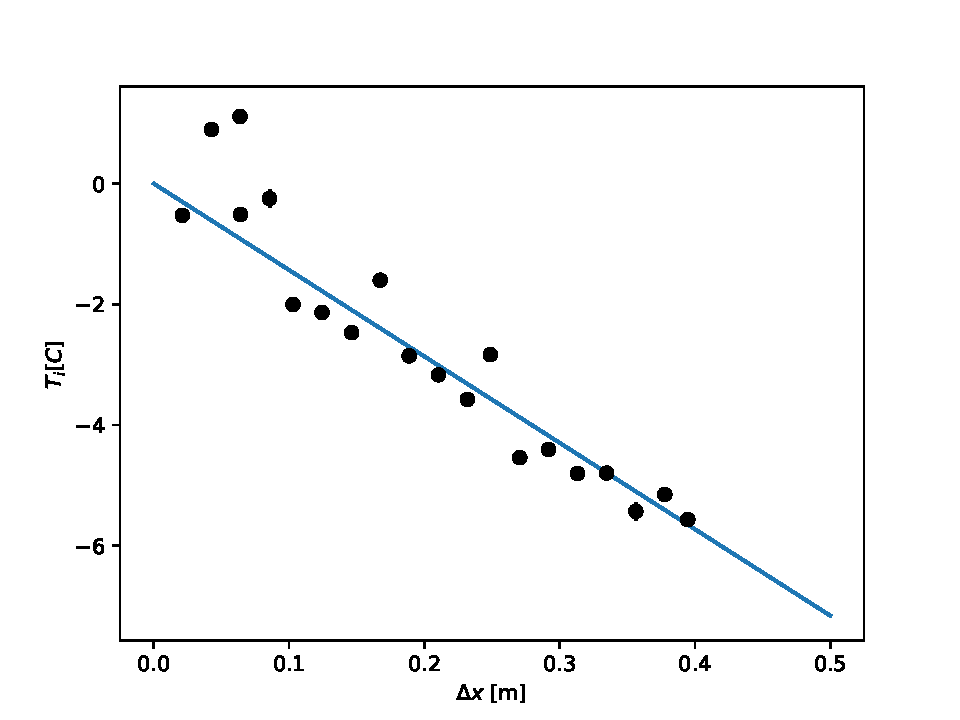
\includegraphics[scale=0.6]{Grafico_differenza_temperatura_rame_dev_scaled.pdf}
\end{minipage}
\hspace{0.01\textwidth}
\begin{minipage}{0.48\textwidth}
	\centering
	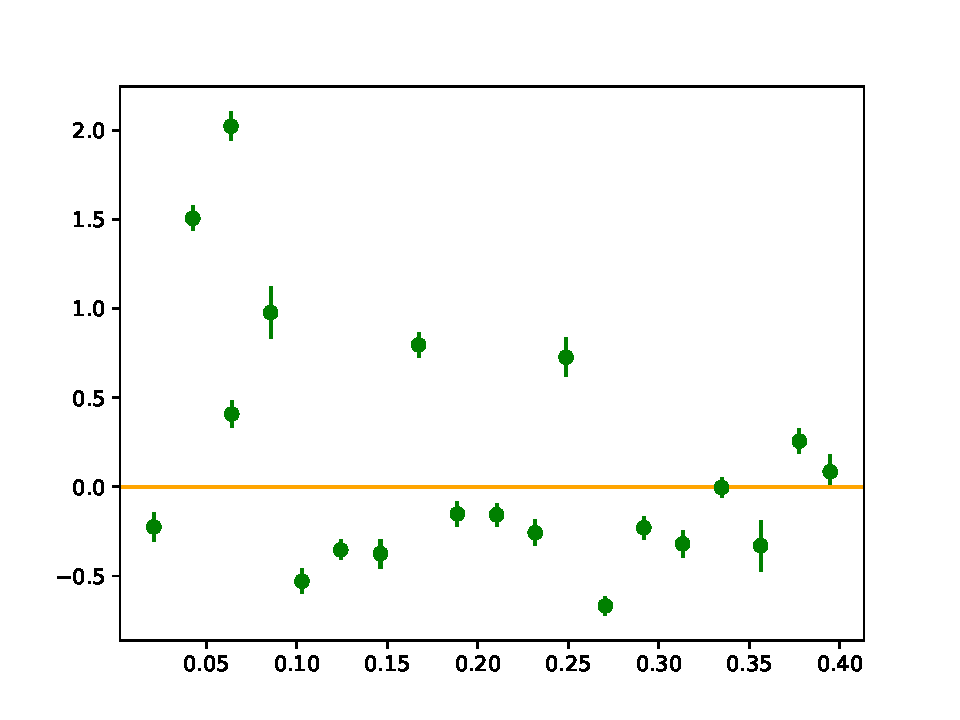
\includegraphics[scale=0.6]{Grafico_residui_rame_dev_scaled.pdf}
\end{minipage}
	\captionof{figure}{Immagine dei nostri grafici in cui si utilizza la deviazione della media aritmetica per stimare le incertezze sulla media delle differenze di temperatura: gli errori sono troppo \emph{piccoli} (fatto che è un evidente sintomo di una stima patologica che sottostima l'incertezza effettiva) e, nel caso specifico di questa immagine, abbiamo moltiplicato di un fattore $4$ gli errori per poterli farli vedere nell'immagine (e nel grafico $\Delta T \, - \, \Delta x$ rimangono comunque poco visibili)}
\end{center}

\noindent Abbiamo anche provato a cercare di stimare le incertezze considerando come incertezza la semidispersione fra la differenza di temperatura più grande misurata e quella minima sperando di ottenere delle stime migliori, tuttavia anche se prendevamo dei grandi \emph{chunk} di dati, la differenza massima e minima erano comunque troppo piccole oppure finivano per coincidere dandoci errore zero, il che è un assurdo. \\
\noindent A riprova del fatto che l'esperimento è dominato dagli errori sistematici, si riporta il valore stimato del $\chi^2$, pari a
\begin{equation*}
	\chi^2 \approx 26860
\end{equation*}
che è un valore troppo alto per i gradi di libertà del nostro esperimento. Inoltre si osserva dal grafico dei residui che i valori non oscillano attorno allo zero, quindi, anche se avessimo trovato un modo per stimare in maniera più accurata gli errori presenti sulle nostre misure, i residui rimarrebbero una prova inattaccabile della presenza di errori sistematici che non possono essere ignorati e mina la validità dell'operazione di \emph{fitting}. \\
Supponendo comunque che le stime effettuate dal fit possano essere comunque ragionevoli e avendo la stima del coefficiente angolare e del suo errore\footnote{riscalando con \texttt{absolute\_sigma=True} la matrice di covarianza} che risulta essere pari a 
\begin{equation}
	m = (-14.9 \pm 1.0) \, \unit{\celsius\per\meter}
\end{equation}
tramite la libreria \emph{scipy} della retta $\hat{m}$ legato alla conducibilità tramite la (\ref{eq:lambda}) abbiamo propagato l'errore su $\lambda$ nella seguente maniera

\begin{equation*}
	\sigma_\lambda = \lambda * \sqrt{ \left( \frac{\sigma_V}{V} \right)^2 + \left( \frac{\sigma_i}{i} \right)^2 + \left( \frac{\sigma_{\hat{m}}}{\hat{m}} \right)^2 + 4 \left(\frac{\sigma_r}{r} \right)^2} 
\end{equation*}
da cui si ricava che
\begin{equation*}
	\lambda = (3.0 \pm 0.2) * 10^2 \, \unit{\watt\per\meter\per\celsius}
\end{equation*}

\noindent che rispetto al valore atteso (sapendo che la conducibilità del rame è $ \tilde \$400 \, \unit{W/m^{-1}°C^{-1}}$) dista circa $5\sigma_{\lambda}$. Sebbene disti relativamente tanto dal valore teorico, potrebbe essere un valore quasi ragionevole considerando tutte le possibili fonte di dissipazioni presenti nella nostra strumentazione. \\
Passiamo adesso all'analisi dei dati dell'alluminio: questi, così come quelli del rame, soffrono sempre il medesimo problema riguardo le incertezze: osservando il grafico del fit (riportato nella pagina successiva) si osserva che, usando la deviazione standard della media, se non fosse per qualche misurazione, avremmo dei dati abbastanza ragionevoli (nel senso di compatibili entro le barre di errore con il modello teorico), tuttavia si osserva dal grafico dei residui che le nostre misure oscillano troppo poco attorno allo zero, il che ci porta a ipotizzare che anche qua siano presenti degli errori sistematici, un fatto diventa ancora più probabile se consideriamo il fatto che la strumentazione e la metodologia usata per le misurazioni dell'alluminio erano le stesse delle misurazioni dell'acciaio.

\begin{center}
\hspace{-1cm}
\begin{minipage}{0.49\textwidth}
	\centering
	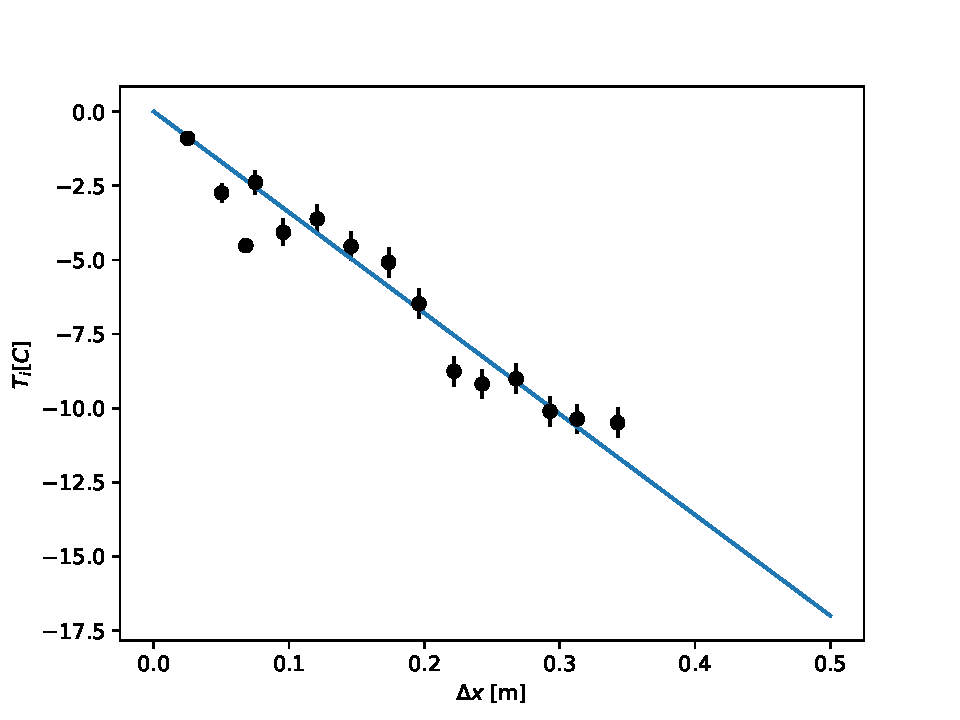
\includegraphics[scale=0.6]{Grafico_differenze_temperatura_alluminio_dev.pdf}
\end{minipage}
\hspace{0.01\textwidth}
\begin{minipage}{0.48\textwidth}
	\centering	
	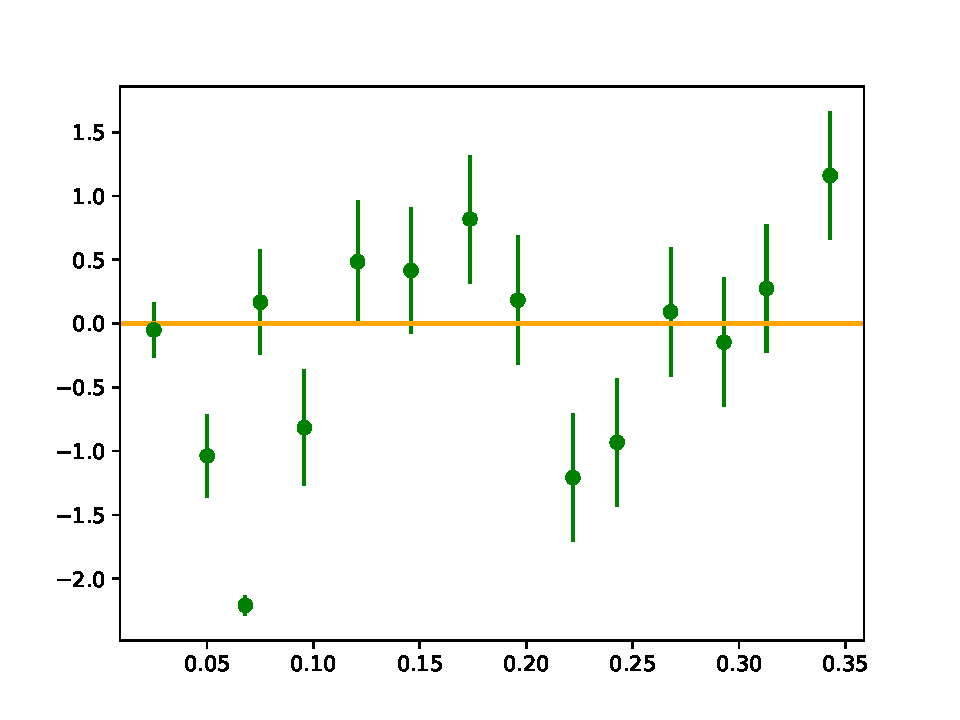
\includegraphics[scale=0.6]{Grafico_residui_alluminio_dev.pdf}
\end{minipage}
\captionof{figure}{Immagine dei grafici e dei residui delle misurazioni effettuate nell'alluminio: sebbene i dati siano più \emph{ragionevoli} tranne per alcuni punti, il grafico dei residui fa ipotizzare che siano presenti ancora degli errori sistematici visto che sono presenti molte permanenze; tesi avvalorata dal fatto che gli strumenti usati e la procedura operativa è rimasta identica a quella usata per la sbarra cilindrica di rame}
\end{center}

\noindent Tuttavia, si osserva dal grafico dei residui che le nostre misure oscillano troppo poco attorno allo zero, il che ci porta a far ipotizzare che anche qua siano presenti errori sistematici, fatto avvalorato dal fatto che le misurazioni con il rame e con l'alluminio sono state effettuate con la stessa strumentazione e la stessa metodologia, pertanto è quasi certo che siano presenti le stesse sorgenti di errori sistematici.	\\
La stima del $\chi^2$ anche qua non produce un risultato molto apprezzabile, anzi, può essere portato nuovamente come prova del fatto che le misure siano completamente dominate dagli errori statistici, infatti questo risulta essere pari a
$$
	\chi^2 \approx 795
$$
che è spropositato rispetto ai gradi di libertà del fit. Osserviamo comunque la stima del coefficiente angolare della retta:
\begin{equation}
	m = (-33 \pm 1) \, \unit{\celsius\per\meter}
\end{equation}
da cui, propagando l'errore come prima, si ottiene che la conducibilità termica è:
\begin{equation}
	\lambda = (126 \pm 5) \, \unit{\watt\per\meter\per\celsius}
\end{equation}
che è dista parecchio dal valore teorico atteso ma, nuovamente, può essere quasi \emph{ragionevole} se consideriamo tutte le possibili fonti di dissipazione del calore.
\newpage
\section{Conclusioni}

L'esperienza non può considerarsi un successo, siccome il risultato che abbiamo ottenuto si discosta di molto dal valore teorico, tuttavia è stata sicuramente un'esperienza istruttiva perché ci ha fatto fare i conti con gli errori sistematici e al fatto che gli esperimenti, quando vengono progettati, devono cercare di ridurre il più possibile gli errori sistematici (per evitare delle situazioni simili a questa esperienza). Nonostante ciò, riteniamo che i valori ottenuti in realtà siano, in realtà, abbastanza \emph{ragionevoli} considerando tutte le possibili fonti di errori sistematici quali le due temperature misurate dai termistori (che possono misurare temperature differenti per eventuali difetti di fabbrica e per le diverse componenti), la dissipazione di energia dalla sbarra, il fatto che la temperatura $T_0$ aumentasse nel tempo e anche il fatto che il circuito che abbiamo usato per riscaldare le sbarre solo idealmente emette una potenza pari a $\frac{VI}{2}$. \\
\end{document}